\chapter{Additional signal and background modelling figures}
\label{app:modelling}

\begin{comment}
\begin{figure}[htp!]
\centering
 \subfloat[RV fits with functional form: DCB$+1$G]{\shortstack{
\includegraphics[width=0.3\textwidth]{modellingFigures/\whichFig/DCBpG/LI/LCtest_ggh_UntaggedTag_0_rv_125.pdf} 
\includegraphics[width=0.3\textwidth]{modellingFigures/\whichFig/DCBpG/LI/LCtest_ggh_UntaggedTag_1_rv_125.pdf} \\
\includegraphics[width=0.3\textwidth]{modellingFigures/\whichFig/DCBpG/LI/LCtest_ggh_UntaggedTag_2_rv_125.pdf} 
\includegraphics[width=0.3\textwidth]{modellingFigures/\whichFig/DCBpG/LI/LCtest_ggh_UntaggedTag_3_rv_125.pdf} 
}}\\
 \subfloat[RV fits with functional form: Sum of Gaussians]{\shortstack{
\includegraphics[width=0.3\textwidth]{modellingFigures/\whichFig/nGaus/LI/LCtest_ggh_UntaggedTag_0_rv_125.pdf} 
\includegraphics[width=0.3\textwidth]{modellingFigures/\whichFig/nGaus/LI/LCtest_ggh_UntaggedTag_1_rv_125.pdf} \\
\includegraphics[width=0.3\textwidth]{modellingFigures/\whichFig/nGaus/LI/LCtest_ggh_UntaggedTag_2_rv_125.pdf} 
\includegraphics[width=0.3\textwidth]{modellingFigures/\whichFig/nGaus/LI/LCtest_ggh_UntaggedTag_3_rv_125.pdf} 
}}\\
\caption{Examples of the shape of the simulated \mgg distribution (\mH=125\GeV) for the ggH process for the \Untagged categories, where the right vertex (RV) was selected. The plots show the agreement between the simulation and the parametrisation expressed as a $\chi^2$, alongside the number of non-empty bins minus the number of parameters in the functional form. Bins with zero entries are ignored in the $\chi^2$ calculation.}
\end{figure}

\clearpage

\begin{figure}[htp!]
\centering
 \subfloat[WV fits with functional form: DCB$+1$G]{\shortstack{
\includegraphics[width=0.3\textwidth]{modellingFigures/\whichFig/DCBpG/LI/LCtest_ggh_UntaggedTag_0_wv_125.pdf} 
\includegraphics[width=0.3\textwidth]{modellingFigures/\whichFig/DCBpG/LI/LCtest_ggh_UntaggedTag_1_wv_125.pdf} \\
\includegraphics[width=0.3\textwidth]{modellingFigures/\whichFig/DCBpG/LI/LCtest_ggh_UntaggedTag_2_wv_125.pdf} 
\includegraphics[width=0.3\textwidth]{modellingFigures/\whichFig/DCBpG/LI/LCtest_ggh_UntaggedTag_3_wv_125.pdf} 
}}\\
 \subfloat[WV fits with functional form: Sum of Gaussians]{\shortstack{
\includegraphics[width=0.3\textwidth]{modellingFigures/\whichFig/nGaus/LI/LCtest_ggh_UntaggedTag_0_wv_125.pdf} 
\includegraphics[width=0.3\textwidth]{modellingFigures/\whichFig/nGaus/LI/LCtest_ggh_UntaggedTag_1_wv_125.pdf} \\
\includegraphics[width=0.3\textwidth]{modellingFigures/\whichFig/nGaus/LI/LCtest_ggh_UntaggedTag_2_wv_125.pdf} 
\includegraphics[width=0.3\textwidth]{modellingFigures/\whichFig/nGaus/LI/LCtest_ggh_UntaggedTag_3_wv_125.pdf} 
}}\\
\caption{Examples of the shape of the simulated \mgg distribution (\mH=125\GeV) for the ggH process for the \Untagged categories, where the wrong vertex (WV) was selected. The plots show the agreement between the simulation and the parametrisation expressed as a $\chi^2$, alongside the number of non-empty bins minus the number of parameters in the functional form. Bins with zero entries are ignored in the $\chi^2$ calculation.}
\end{figure}

\clearpage
\begin{figure}[htp!]
\centering
 \subfloat[RV fits with functional form: DCB$+1$G]{\shortstack{
\includegraphics[width=0.3\textwidth]{modellingFigures/\whichFig/DCBpG/LI/LCtest_ggh_VBFTag_0_rv_125.pdf} 
\includegraphics[width=0.3\textwidth]{modellingFigures/\whichFig/DCBpG/LI/LCtest_ggh_VBFTag_1_rv_125.pdf} \\
\includegraphics[width=0.3\textwidth]{modellingFigures/\whichFig/DCBpG/LI/LCtest_ggh_TTHHadronicTag_rv_125.pdf} 
\includegraphics[width=0.3\textwidth]{modellingFigures/\whichFig/DCBpG/LI/LCtest_ggh_TTHLeptonicTag_rv_125.pdf} 
}}\\
 \subfloat[RV fits with functional form: Sum of Gaussians]{\shortstack{
\includegraphics[width=0.3\textwidth]{modellingFigures/\whichFig/nGaus/LI/LCtest_ggh_VBFTag_0_rv_125.pdf} 
\includegraphics[width=0.3\textwidth]{modellingFigures/\whichFig/nGaus/LI/LCtest_ggh_VBFTag_1_rv_125.pdf} \\
\includegraphics[width=0.3\textwidth]{modellingFigures/\whichFig/nGaus/LI/LCtest_ggh_TTHHadronicTag_rv_125.pdf} 
\includegraphics[width=0.3\textwidth]{modellingFigures/\whichFig/nGaus/LI/LCtest_ggh_TTHLeptonicTag_rv_125.pdf} 
}}\\
\caption{Examples of the shape of the simulated \mgg distribution (\mH=125\GeV) for the ggH process for the \VBFTag and \TTHTag categories, where the right vertex (RV) was selected. The plots show the agreement between the simulation and the parametrisation expressed as a $\chi^2$, alongside the number of non-empty bins minus the number of parameters in the functional form. Bins with zero entries are ignored in the $\chi^2$ calculation.}
\end{figure}

\clearpage
\begin{figure}[htp!]
\centering
 \subfloat[WV fits with functional form: DCB$+1$G]{\shortstack{
\includegraphics[width=0.3\textwidth]{modellingFigures/\whichFig/DCBpG/LI/LCtest_ggh_VBFTag_0_wv_125.pdf} 
\includegraphics[width=0.3\textwidth]{modellingFigures/\whichFig/DCBpG/LI/LCtest_ggh_VBFTag_1_wv_125.pdf} \\
\includegraphics[width=0.3\textwidth]{modellingFigures/\whichFig/DCBpG/LI/LCtest_ggh_TTHHadronicTag_wv_125.pdf} 
\includegraphics[width=0.3\textwidth]{modellingFigures/\whichFig/DCBpG/LI/LCtest_ggh_TTHLeptonicTag_wv_125.pdf} 
}}\\
 \subfloat[WV fits with functional form: Sum of Gaussians]{\shortstack{
\includegraphics[width=0.3\textwidth]{modellingFigures/\whichFig/nGaus/LI/LCtest_ggh_VBFTag_0_wv_125.pdf} 
\includegraphics[width=0.3\textwidth]{modellingFigures/\whichFig/nGaus/LI/LCtest_ggh_VBFTag_1_wv_125.pdf} \\
\includegraphics[width=0.3\textwidth]{modellingFigures/\whichFig/nGaus/LI/LCtest_ggh_TTHHadronicTag_wv_125.pdf} 
\includegraphics[width=0.3\textwidth]{modellingFigures/\whichFig/nGaus/LI/LCtest_ggh_TTHLeptonicTag_wv_125.pdf} 
}}\\
\caption{Examples of the shape of the simulated \mgg distribution (\mH=125\GeV) for the ggH process for the \VBFTag and \TTHTag categories, where the wrong vertex (WV) was selected. The plots show the agreement between the simulation and the parametrisation expressed as a $\chi^2$, alongside the number of non-empty bins minus the number of parameters in the functional form. Bins with zero entries are ignored in the $\chi^2$ calculation.}
\end{figure}


\begin{figure}[htp!]
\centering
 \subfloat[RV fits with functional form: DCB$+1$G]{\shortstack{
\includegraphics[width=0.3\textwidth]{modellingFigures/\whichFig/DCBpG/LI/LCtest_vbf_UntaggedTag_0_rv_125.pdf} 
\includegraphics[width=0.3\textwidth]{modellingFigures/\whichFig/DCBpG/LI/LCtest_vbf_UntaggedTag_1_rv_125.pdf} \\
\includegraphics[width=0.3\textwidth]{modellingFigures/\whichFig/DCBpG/LI/LCtest_vbf_UntaggedTag_2_rv_125.pdf} 
\includegraphics[width=0.3\textwidth]{modellingFigures/\whichFig/DCBpG/LI/LCtest_vbf_UntaggedTag_3_rv_125.pdf} 
}}\\
 \subfloat[RV fits with functional form: Sum of Gaussians]{\shortstack{
\includegraphics[width=0.3\textwidth]{modellingFigures/\whichFig/nGaus/LI/LCtest_vbf_UntaggedTag_0_rv_125.pdf} 
\includegraphics[width=0.3\textwidth]{modellingFigures/\whichFig/nGaus/LI/LCtest_vbf_UntaggedTag_1_rv_125.pdf} \\
\includegraphics[width=0.3\textwidth]{modellingFigures/\whichFig/nGaus/LI/LCtest_vbf_UntaggedTag_2_rv_125.pdf} 
\includegraphics[width=0.3\textwidth]{modellingFigures/\whichFig/nGaus/LI/LCtest_vbf_UntaggedTag_3_rv_125.pdf} 
}}\\
\caption{Examples of the shape of the simulated \mgg distribution (\mH=125\GeV) for the VBF process for the \Untagged categories, where the right vertex (RV) was selected. The plots show the agreement between the simulation and the parametrisation expressed as a $\chi^2$, alongside the number of non-empty bins minus the number of parameters in the functional form. Bins with zero entries are ignored in the $\chi^2$ calculation.}
\end{figure}

\clearpage
\begin{figure}[htp!]
\centering
 \subfloat[WV fits with functional form: DCB$+1$G]{\shortstack{
\includegraphics[width=0.3\textwidth]{modellingFigures/\whichFig/DCBpG/LI/LCtest_vbf_UntaggedTag_0_wv_125.pdf} 
\includegraphics[width=0.3\textwidth]{modellingFigures/\whichFig/DCBpG/LI/LCtest_vbf_UntaggedTag_1_wv_125.pdf} \\
\includegraphics[width=0.3\textwidth]{modellingFigures/\whichFig/DCBpG/LI/LCtest_vbf_UntaggedTag_2_wv_125.pdf} 
\includegraphics[width=0.3\textwidth]{modellingFigures/\whichFig/DCBpG/LI/LCtest_vbf_UntaggedTag_3_wv_125.pdf} 
}}\\
 \subfloat[WV fits with functional form: Sum of Gaussians]{\shortstack{
\includegraphics[width=0.3\textwidth]{modellingFigures/\whichFig/nGaus/LI/LCtest_vbf_UntaggedTag_0_wv_125.pdf} 
\includegraphics[width=0.3\textwidth]{modellingFigures/\whichFig/nGaus/LI/LCtest_vbf_UntaggedTag_1_wv_125.pdf} \\
\includegraphics[width=0.3\textwidth]{modellingFigures/\whichFig/nGaus/LI/LCtest_vbf_UntaggedTag_2_wv_125.pdf} 
\includegraphics[width=0.3\textwidth]{modellingFigures/\whichFig/nGaus/LI/LCtest_vbf_UntaggedTag_3_wv_125.pdf} 
}}\\
\caption{Examples of the shape of the simulated \mgg distribution (\mH=125\GeV) for the VBF process for the \Untagged categories, where the wrong vertex (WV) was selected. The plots show the agreement between the simulation and the parametrisation expressed as a $\chi^2$, alongside the number of non-empty bins minus the number of parameters in the functional form. Bins with zero entries are ignored in the $\chi^2$ calculation.}
\end{figure}

\clearpage
\begin{figure}[htp!]
\centering
 \subfloat[RV fits with functional form: DCB$+1$G]{\shortstack{
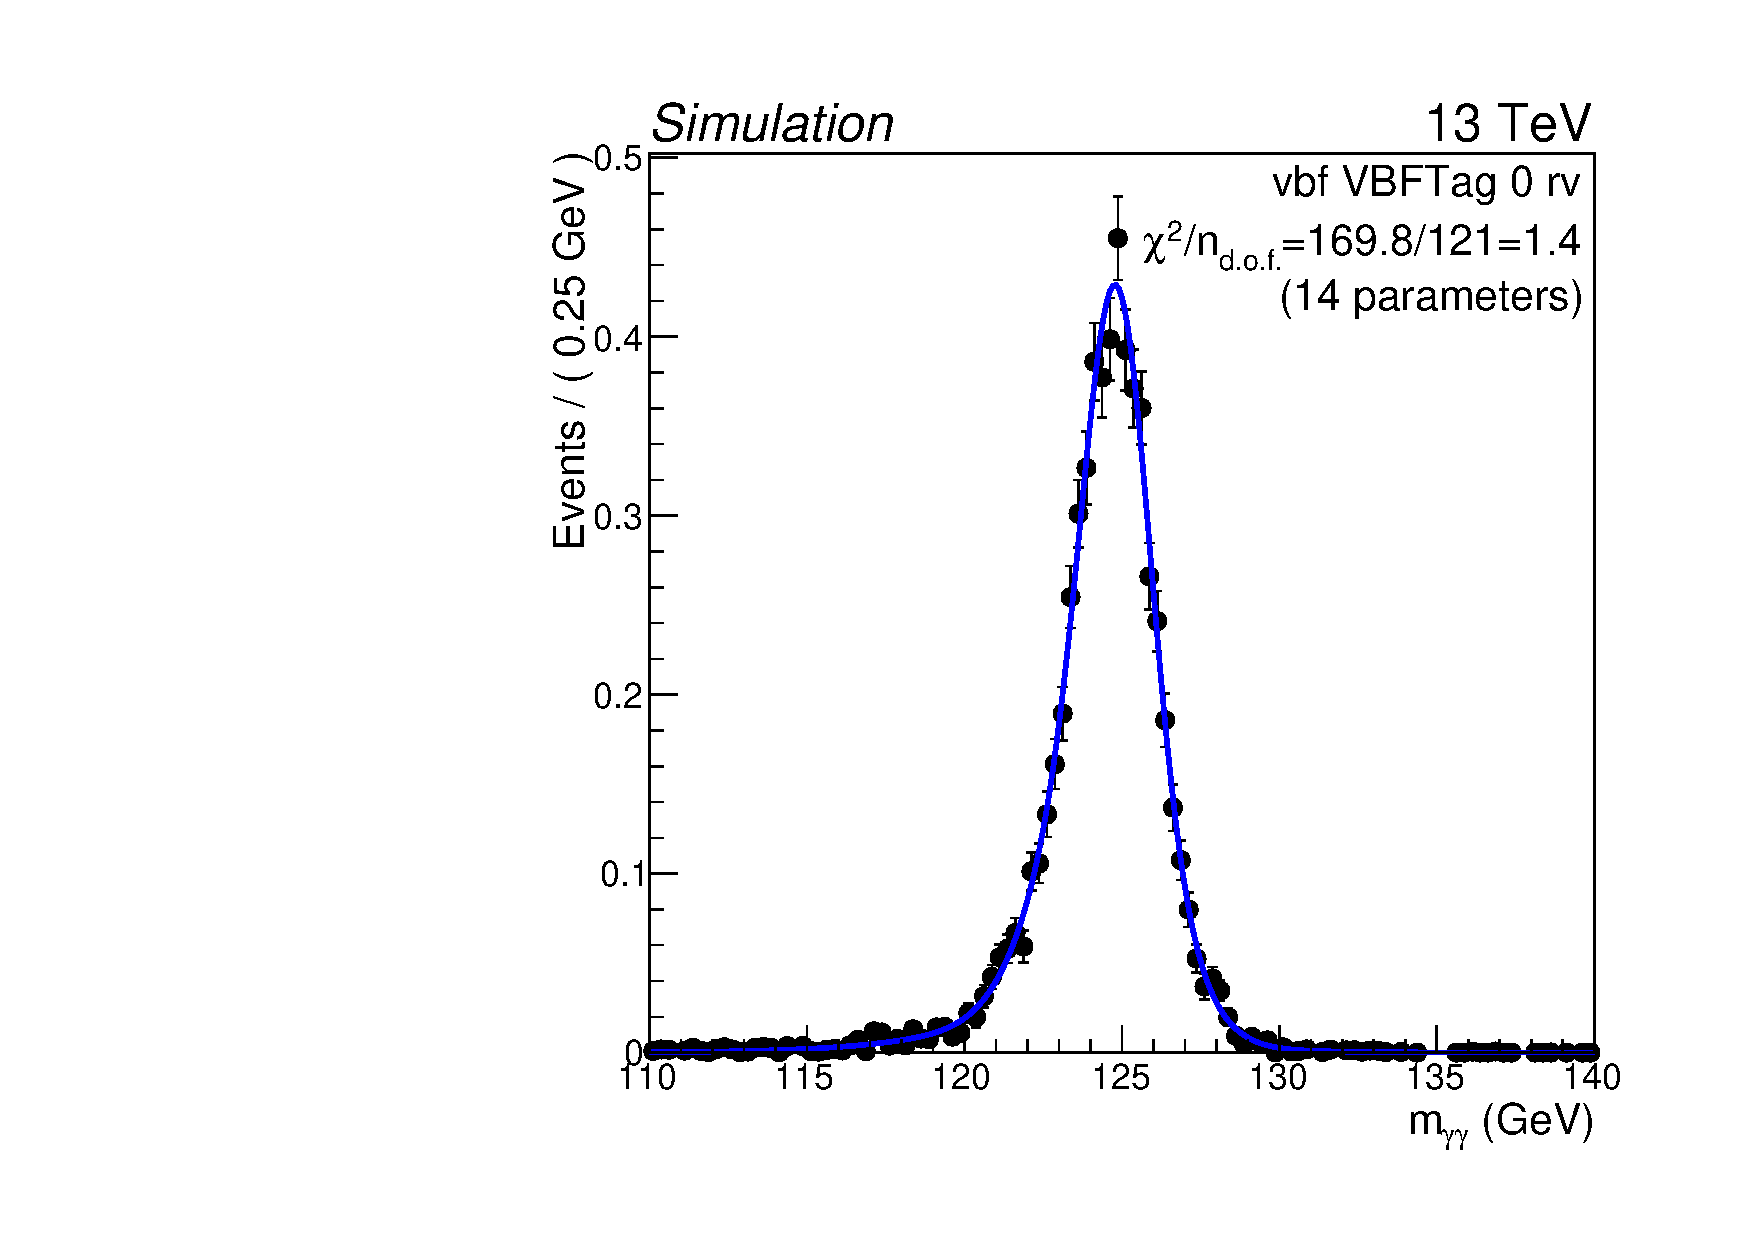
\includegraphics[width=0.3\textwidth]{modellingFigures/\whichFig/DCBpG/LI/LCtest_vbf_VBFTag_0_rv_125.pdf} 
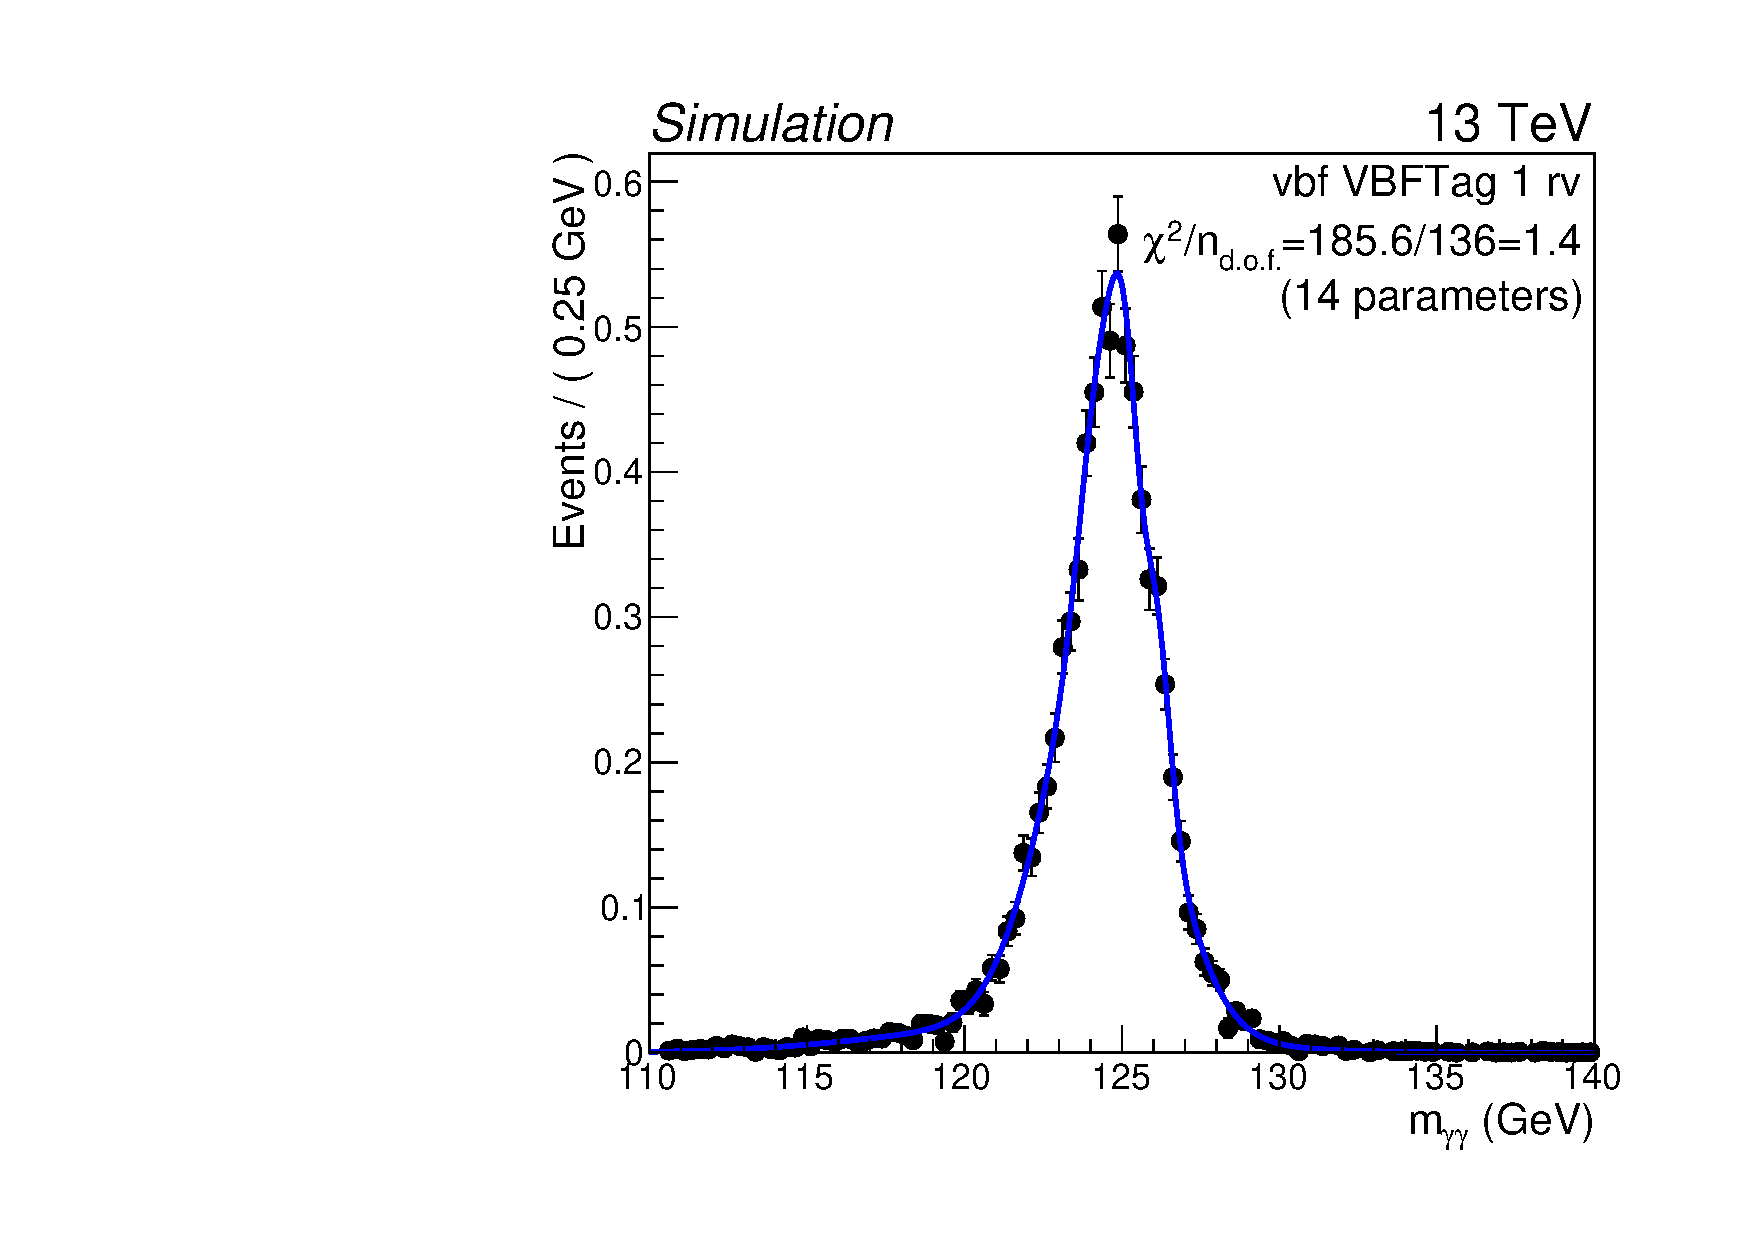
\includegraphics[width=0.3\textwidth]{modellingFigures/\whichFig/DCBpG/LI/LCtest_vbf_VBFTag_1_rv_125.pdf} \\
\includegraphics[width=0.3\textwidth]{modellingFigures/\whichFig/DCBpG/LI/LCtest_vbf_TTHHadronicTag_rv_125.pdf} 
\includegraphics[width=0.3\textwidth]{modellingFigures/\whichFig/DCBpG/LI/LCtest_vbf_TTHLeptonicTag_rv_125.pdf} 
}}\\
 \subfloat[RV fits with functional form: Sum of Gaussians]{\shortstack{
\includegraphics[width=0.3\textwidth]{modellingFigures/\whichFig/nGaus/LI/LCtest_vbf_VBFTag_0_rv_125.pdf} 
\includegraphics[width=0.3\textwidth]{modellingFigures/\whichFig/nGaus/LI/LCtest_vbf_VBFTag_1_rv_125.pdf} \\
\includegraphics[width=0.3\textwidth]{modellingFigures/\whichFig/nGaus/LI/LCtest_vbf_TTHHadronicTag_rv_125.pdf} 
\includegraphics[width=0.3\textwidth]{modellingFigures/\whichFig/nGaus/LI/LCtest_vbf_TTHLeptonicTag_rv_125.pdf} 
}}\\
\caption{Examples of the shape of the simulated \mgg distribution (\mH=125\GeV) for the VBF process for the \VBFTag and \TTHTag categories, where the right vertex (RV) was selected. The plots show the agreement between the simulation and the parametrisation expressed as a $\chi^2$, alongside the number of non-empty bins minus the number of parameters in the functional form. Bins with zero entries are ignored in the $\chi^2$ calculation.}
\end{figure}


\clearpage
\begin{figure}[htp!]
\centering
 \subfloat[WV fits with functional form: DCB$+1$G]{\shortstack{
\includegraphics[width=0.3\textwidth]{modellingFigures/\whichFig/DCBpG/LI/LCtest_vbf_VBFTag_0_wv_125.pdf} 
\includegraphics[width=0.3\textwidth]{modellingFigures/\whichFig/DCBpG/LI/LCtest_vbf_VBFTag_1_wv_125.pdf} \\
\includegraphics[width=0.3\textwidth]{modellingFigures/\whichFig/DCBpG/LI/LCtest_vbf_TTHHadronicTag_wv_125.pdf} 
\includegraphics[width=0.3\textwidth]{modellingFigures/\whichFig/DCBpG/LI/LCtest_vbf_TTHLeptonicTag_wv_125.pdf} 
}}\\
 \subfloat[WV fits with functional form: Sum of Gaussians]{\shortstack{
\includegraphics[width=0.3\textwidth]{modellingFigures/\whichFig/nGaus/LI/LCtest_vbf_VBFTag_0_wv_125.pdf} 
\includegraphics[width=0.3\textwidth]{modellingFigures/\whichFig/nGaus/LI/LCtest_vbf_VBFTag_1_wv_125.pdf} \\
\includegraphics[width=0.3\textwidth]{modellingFigures/\whichFig/nGaus/LI/LCtest_vbf_TTHHadronicTag_wv_125.pdf} 
\includegraphics[width=0.3\textwidth]{modellingFigures/\whichFig/nGaus/LI/LCtest_vbf_TTHLeptonicTag_wv_125.pdf} 
}}\\
\caption{Examples of the shape of the simulated \mgg distribution (\mH=125\GeV) for the VBF process for the \VBFTag and \TTHTag categories, where the wrong vertex (WV) was selected. The plots show the agreement between the simulation and the parametrisation expressed as a $\chi^2$, alongside the number of non-empty bins minus the number of parameters in the functional form. Bins with zero entries are ignored in the $\chi^2$ calculation.}
\end{figure}


\begin{figure}[htp!]
\centering
 \subfloat[RV fits with functional form: DCB$+1$G]{\shortstack{
\includegraphics[width=0.3\textwidth]{modellingFigures/\whichFig/DCBpG/LI/LCtest_tth_UntaggedTag_0_rv_125.pdf} 
\includegraphics[width=0.3\textwidth]{modellingFigures/\whichFig/DCBpG/LI/LCtest_tth_UntaggedTag_1_rv_125.pdf} \\
\includegraphics[width=0.3\textwidth]{modellingFigures/\whichFig/DCBpG/LI/LCtest_tth_UntaggedTag_2_rv_125.pdf} 
\includegraphics[width=0.3\textwidth]{modellingFigures/\whichFig/DCBpG/LI/LCtest_tth_UntaggedTag_3_rv_125.pdf} 
}}\\
 \subfloat[RV fits with functional form: Sum of Gaussians]{\shortstack{
\includegraphics[width=0.3\textwidth]{modellingFigures/\whichFig/nGaus/LI/LCtest_tth_UntaggedTag_0_rv_125.pdf} 
\includegraphics[width=0.3\textwidth]{modellingFigures/\whichFig/nGaus/LI/LCtest_tth_UntaggedTag_1_rv_125.pdf} \\
\includegraphics[width=0.3\textwidth]{modellingFigures/\whichFig/nGaus/LI/LCtest_tth_UntaggedTag_2_rv_125.pdf} 
\includegraphics[width=0.3\textwidth]{modellingFigures/\whichFig/nGaus/LI/LCtest_tth_UntaggedTag_3_rv_125.pdf} 
}}\\
\caption{Examples of the shape of the simulated \mgg distribution (\mH=125\GeV) for the ttH process for the \Untagged categories, where the right vertex (RV) was selected. The plots show the agreement between the simulation and the parametrisation expressed as a $\chi^2$, alongside the number of non-empty bins minus the number of parameters in the functional form. Bins with zero entries are ignored in the $\chi^2$ calculation.}
\end{figure}

\clearpage
\begin{figure}[htp!]
\centering
 \subfloat[WV fits with functional form: DCB$+1$G]{\shortstack{
\includegraphics[width=0.3\textwidth]{modellingFigures/\whichFig/DCBpG/LI/LCtest_tth_UntaggedTag_0_wv_125.pdf} 
\includegraphics[width=0.3\textwidth]{modellingFigures/\whichFig/DCBpG/LI/LCtest_tth_UntaggedTag_1_wv_125.pdf} \\
\includegraphics[width=0.3\textwidth]{modellingFigures/\whichFig/DCBpG/LI/LCtest_tth_UntaggedTag_2_wv_125.pdf} 
\includegraphics[width=0.3\textwidth]{modellingFigures/\whichFig/DCBpG/LI/LCtest_tth_UntaggedTag_3_wv_125.pdf} 
}}\\
 \subfloat[WV fits with functional form: Sum of Gaussians]{\shortstack{
\includegraphics[width=0.3\textwidth]{modellingFigures/\whichFig/nGaus/LI/LCtest_tth_UntaggedTag_0_wv_125.pdf} 
\includegraphics[width=0.3\textwidth]{modellingFigures/\whichFig/nGaus/LI/LCtest_tth_UntaggedTag_1_wv_125.pdf} \\
\includegraphics[width=0.3\textwidth]{modellingFigures/\whichFig/nGaus/LI/LCtest_tth_UntaggedTag_2_wv_125.pdf} 
\includegraphics[width=0.3\textwidth]{modellingFigures/\whichFig/nGaus/LI/LCtest_tth_UntaggedTag_3_wv_125.pdf} 
}}\\
\caption{Examples of the shape of the simulated \mgg distribution (\mH=125\GeV) for the ttH process for the \Untagged categories, where the wrong vertex (WV) was selected. The plots show the agreement between the simulation and the parametrisation expressed as a $\chi^2$, alongside the number of non-empty bins minus the number of parameters in the functional form. Bins with zero entries are ignored in the $\chi^2$ calculation.}
\end{figure}

\begin{figure}[htp!]
\centering
 \subfloat[RV fits with functional form: DCB$+1$G]{\shortstack{
\includegraphics[width=0.3\textwidth]{modellingFigures/\whichFig/DCBpG/LI/LCtest_tth_VBFTag_0_rv_125.pdf} 
\includegraphics[width=0.3\textwidth]{modellingFigures/\whichFig/DCBpG/LI/LCtest_tth_VBFTag_1_rv_125.pdf} \\
\includegraphics[width=0.3\textwidth]{modellingFigures/\whichFig/DCBpG/LI/LCtest_tth_TTHHadronicTag_rv_125.pdf} 
\includegraphics[width=0.3\textwidth]{modellingFigures/\whichFig/DCBpG/LI/LCtest_tth_TTHLeptonicTag_rv_125.pdf} 
}}\\
 \subfloat[RV fits with functional form: Sum of Gaussians]{\shortstack{
\includegraphics[width=0.3\textwidth]{modellingFigures/\whichFig/nGaus/LI/LCtest_tth_VBFTag_0_rv_125.pdf} 
\includegraphics[width=0.3\textwidth]{modellingFigures/\whichFig/nGaus/LI/LCtest_tth_VBFTag_1_rv_125.pdf} \\
\includegraphics[width=0.3\textwidth]{modellingFigures/\whichFig/nGaus/LI/LCtest_tth_TTHHadronicTag_rv_125.pdf} 
\includegraphics[width=0.3\textwidth]{modellingFigures/\whichFig/nGaus/LI/LCtest_tth_TTHLeptonicTag_rv_125.pdf} 
}}\\
\caption{Examples of the shape of the simulated \mgg distribution (\mH=125\GeV) for the ttH process for the \VBFTag and \TTHTag categories, where the right vertex (RV) was selected. The plots show the agreement between the simulation and the parametrisation expressed as a $\chi^2$, alongside the number of non-empty bins minus the number of parameters in the functional form. Bins with zero entries are ignored in the $\chi^2$ calculation.}
\end{figure}

\clearpage
\begin{figure}[htp!]
\centering
 \subfloat[WV fits with functional form: DCB$+1$G]{\shortstack{
\includegraphics[width=0.3\textwidth]{modellingFigures/\whichFig/DCBpG/LI/LCtest_tth_VBFTag_0_wv_125.pdf} 
\includegraphics[width=0.3\textwidth]{modellingFigures/\whichFig/DCBpG/LI/LCtest_tth_VBFTag_1_wv_125.pdf} \\
\includegraphics[width=0.3\textwidth]{modellingFigures/\whichFig/DCBpG/LI/LCtest_tth_TTHHadronicTag_wv_125.pdf} 
\includegraphics[width=0.3\textwidth]{modellingFigures/\whichFig/DCBpG/LI/LCtest_tth_TTHLeptonicTag_wv_125.pdf} 
}}\\
 \subfloat[WV fits with functional form: Sum of Gaussians]{\shortstack{
\includegraphics[width=0.3\textwidth]{modellingFigures/\whichFig/nGaus/LI/LCtest_tth_VBFTag_0_wv_125.pdf} 
\includegraphics[width=0.3\textwidth]{modellingFigures/\whichFig/nGaus/LI/LCtest_tth_VBFTag_1_wv_125.pdf} \\
\includegraphics[width=0.3\textwidth]{modellingFigures/\whichFig/nGaus/LI/LCtest_tth_TTHHadronicTag_wv_125.pdf} 
\includegraphics[width=0.3\textwidth]{modellingFigures/\whichFig/nGaus/LI/LCtest_tth_TTHLeptonicTag_wv_125.pdf} 
}}\\
\caption{Examples of the shape of the simulated \mgg distribution (\mH=125\GeV) for the ttH process for the \VBFTag and \TTHTag categories, where the wrong vertex (WV) was selected. The plots show the agreement between the simulation and the parametrisation expressed as a $\chi^2$, alongside the number of non-empty bins minus the number of parameters in the functional form. Bins with zero entries are ignored in the $\chi^2$ calculation.}
\end{figure}

\clearpage

\begin{figure}[htp!]
\centering
 \subfloat[RV fits with functional form: DCB$+1$G]{\shortstack{
\includegraphics[width=0.3\textwidth]{modellingFigures/\whichFig/DCBpG/LI/LCtest_wh_UntaggedTag_0_rv_125.pdf} 
\includegraphics[width=0.3\textwidth]{modellingFigures/\whichFig/DCBpG/LI/LCtest_wh_UntaggedTag_1_rv_125.pdf} \\
\includegraphics[width=0.3\textwidth]{modellingFigures/\whichFig/DCBpG/LI/LCtest_wh_UntaggedTag_2_rv_125.pdf} 
\includegraphics[width=0.3\textwidth]{modellingFigures/\whichFig/DCBpG/LI/LCtest_wh_UntaggedTag_3_rv_125.pdf} 
}}\\
 \subfloat[RV fits with functional form: Sum of Gaussians]{\shortstack{
\includegraphics[width=0.3\textwidth]{modellingFigures/\whichFig/nGaus/LI/LCtest_wh_UntaggedTag_0_rv_125.pdf} 
\includegraphics[width=0.3\textwidth]{modellingFigures/\whichFig/nGaus/LI/LCtest_wh_UntaggedTag_1_rv_125.pdf} \\
\includegraphics[width=0.3\textwidth]{modellingFigures/\whichFig/nGaus/LI/LCtest_wh_UntaggedTag_2_rv_125.pdf} 
\includegraphics[width=0.3\textwidth]{modellingFigures/\whichFig/nGaus/LI/LCtest_wh_UntaggedTag_3_rv_125.pdf} 
}}\\
\caption{Examples of the shape of the simulated \mgg distribution (\mH=125\GeV) for the WH process for the \Untagged categories, where the right vertex (RV) was selected. The plots show the agreement between the simulation and the parametrisation expressed as a $\chi^2$, alongside the number of non-empty bins minus the number of parameters in the functional form. Bins with zero entries are ignored in the $\chi^2$ calculation.}
\end{figure}

\begin{figure}[htp!]
\centering
 \subfloat[WV fits with functional form: DCB$+1$G]{\shortstack{
\includegraphics[width=0.3\textwidth]{modellingFigures/\whichFig/DCBpG/LI/LCtest_wh_UntaggedTag_0_wv_125.pdf} 
\includegraphics[width=0.3\textwidth]{modellingFigures/\whichFig/DCBpG/LI/LCtest_wh_UntaggedTag_1_wv_125.pdf} \\
\includegraphics[width=0.3\textwidth]{modellingFigures/\whichFig/DCBpG/LI/LCtest_wh_UntaggedTag_2_wv_125.pdf} 
\includegraphics[width=0.3\textwidth]{modellingFigures/\whichFig/DCBpG/LI/LCtest_wh_UntaggedTag_3_wv_125.pdf} 
}}\\
 \subfloat[WV fits with functional form: Sum of Gaussians]{\shortstack{
\includegraphics[width=0.3\textwidth]{modellingFigures/\whichFig/nGaus/LI/LCtest_wh_UntaggedTag_0_wv_125.pdf} 
\includegraphics[width=0.3\textwidth]{modellingFigures/\whichFig/nGaus/LI/LCtest_wh_UntaggedTag_1_wv_125.pdf} \\
\includegraphics[width=0.3\textwidth]{modellingFigures/\whichFig/nGaus/LI/LCtest_wh_UntaggedTag_2_wv_125.pdf} 
\includegraphics[width=0.3\textwidth]{modellingFigures/\whichFig/nGaus/LI/LCtest_wh_UntaggedTag_3_wv_125.pdf} 
}}\\
\caption{Examples of the shape of the simulated \mgg distribution (\mH=125\GeV) for the WH process for the \Untagged categories, where the wrong vertex (WV) was selected. The plots show the agreement between the simulation and the parametrisation expressed as a $\chi^2$, alongside the number of non-empty bins minus the number of parameters in the functional form. Bins with zero entries are ignored in the $\chi^2$ calculation.}
\end{figure}

\clearpage
\begin{figure}[htp!]
\centering
 \subfloat[RV fits with functional form: DCB$+1$G]{\shortstack{
\includegraphics[width=0.3\textwidth]{modellingFigures/\whichFig/DCBpG/LI/LCtest_wh_VBFTag_0_rv_125.pdf} 
\includegraphics[width=0.3\textwidth]{modellingFigures/\whichFig/DCBpG/LI/LCtest_wh_VBFTag_1_rv_125.pdf} \\
\includegraphics[width=0.3\textwidth]{modellingFigures/\whichFig/DCBpG/LI/LCtest_wh_TTHHadronicTag_rv_125.pdf} 
\includegraphics[width=0.3\textwidth]{modellingFigures/\whichFig/DCBpG/LI/LCtest_wh_TTHLeptonicTag_rv_125.pdf} 
}}\\
 \subfloat[RV fits with functional form: Sum of Gaussians]{\shortstack{
\includegraphics[width=0.3\textwidth]{modellingFigures/\whichFig/nGaus/LI/LCtest_wh_VBFTag_0_rv_125.pdf} 
\includegraphics[width=0.3\textwidth]{modellingFigures/\whichFig/nGaus/LI/LCtest_wh_VBFTag_1_rv_125.pdf} \\
\includegraphics[width=0.3\textwidth]{modellingFigures/\whichFig/nGaus/LI/LCtest_wh_TTHHadronicTag_rv_125.pdf} 
\includegraphics[width=0.3\textwidth]{modellingFigures/\whichFig/nGaus/LI/LCtest_wh_TTHLeptonicTag_rv_125.pdf} 
}}\\
\caption{Examples of the shape of the simulated \mgg distribution (\mH=125\GeV) for the WH process for the \VBFTag and \TTHTag categories, where the right vertex (RV) was selected. The plots show the agreement between the simulation and the parametrisation expressed as a $\chi^2$, alongside the number of non-empty bins minus the number of parameters in the functional form. Bins with zero entries are ignored in the $\chi^2$ calculation.}
\end{figure}

\begin{figure}[htp!]
\centering
 \subfloat[WV fits with functional form: DCB$+1$G]{\shortstack{
\includegraphics[width=0.3\textwidth]{modellingFigures/\whichFig/DCBpG/LI/LCtest_wh_VBFTag_0_wv_125.pdf} 
\includegraphics[width=0.3\textwidth]{modellingFigures/\whichFig/DCBpG/LI/LCtest_wh_VBFTag_1_wv_125.pdf} \\
\includegraphics[width=0.3\textwidth]{modellingFigures/\whichFig/DCBpG/LI/LCtest_wh_TTHHadronicTag_wv_125.pdf} 
\includegraphics[width=0.3\textwidth]{modellingFigures/\whichFig/DCBpG/LI/LCtest_wh_TTHLeptonicTag_wv_125.pdf} 
}}\\
 \subfloat[WV fits with functional form: Sum of Gaussians]{\shortstack{
\includegraphics[width=0.3\textwidth]{modellingFigures/\whichFig/nGaus/LI/LCtest_wh_VBFTag_0_wv_125.pdf} 
\includegraphics[width=0.3\textwidth]{modellingFigures/\whichFig/nGaus/LI/LCtest_wh_VBFTag_1_wv_125.pdf} \\
\includegraphics[width=0.3\textwidth]{modellingFigures/\whichFig/nGaus/LI/LCtest_wh_TTHHadronicTag_wv_125.pdf} 
\includegraphics[width=0.3\textwidth]{modellingFigures/\whichFig/nGaus/LI/LCtest_wh_TTHLeptonicTag_wv_125.pdf} 
}}\\
\caption{Examples of the shape of the simulated \mgg distribution (\mH=125\GeV) for the WH process for the \VBFTag and \TTHTag categories, where the wrong vertex (WV) was selected. The plots show the agreement between the simulation and the parametrisation expressed as a $\chi^2$, alongside the number of non-empty bins minus the number of parameters in the functional form. Bins with zero entries are ignored in the $\chi^2$ calculation.}
\end{figure}


\clearpage


\begin{figure}[htp!]
\centering
 \subfloat[RV fits with functional form: DCB$+1$G]{\shortstack{
\includegraphics[width=0.3\textwidth]{modellingFigures/\whichFig/DCBpG/LI/LCtest_zh_UntaggedTag_0_rv_125.pdf} 
\includegraphics[width=0.3\textwidth]{modellingFigures/\whichFig/DCBpG/LI/LCtest_zh_UntaggedTag_1_rv_125.pdf} \\
\includegraphics[width=0.3\textwidth]{modellingFigures/\whichFig/DCBpG/LI/LCtest_zh_UntaggedTag_2_rv_125.pdf} 
\includegraphics[width=0.3\textwidth]{modellingFigures/\whichFig/DCBpG/LI/LCtest_zh_UntaggedTag_3_rv_125.pdf} 
}}\\
 \subfloat[RV fits with functional form: Sum of Gaussians]{\shortstack{
\includegraphics[width=0.3\textwidth]{modellingFigures/\whichFig/nGaus/LI/LCtest_zh_UntaggedTag_0_rv_125.pdf} 
\includegraphics[width=0.3\textwidth]{modellingFigures/\whichFig/nGaus/LI/LCtest_zh_UntaggedTag_1_rv_125.pdf} \\
\includegraphics[width=0.3\textwidth]{modellingFigures/\whichFig/nGaus/LI/LCtest_zh_UntaggedTag_2_rv_125.pdf} 
\includegraphics[width=0.3\textwidth]{modellingFigures/\whichFig/nGaus/LI/LCtest_zh_UntaggedTag_3_rv_125.pdf} 
}}\\
\caption{Examples of the shape of the simulated \mgg distribution (\mH=125\GeV) for the ZH process for the \Untagged categories, where the right vertex (RV) was selected. The plots show the agreement between the simulation and the parametrisation expressed as a $\chi^2$, alongside the number of non-empty bins minus the number of parameters in the functional form. Bins with zero entries are ignored in the $\chi^2$ calculation.}
\end{figure}

\clearpage
\begin{figure}[htp!]
\centering
 \subfloat[WV fits with functional form: DCB$+1$G]{\shortstack{
\includegraphics[width=0.3\textwidth]{modellingFigures/\whichFig/DCBpG/LI/LCtest_zh_UntaggedTag_0_wv_125.pdf} 
\includegraphics[width=0.3\textwidth]{modellingFigures/\whichFig/DCBpG/LI/LCtest_zh_UntaggedTag_1_wv_125.pdf} \\
\includegraphics[width=0.3\textwidth]{modellingFigures/\whichFig/DCBpG/LI/LCtest_zh_UntaggedTag_2_wv_125.pdf} 
\includegraphics[width=0.3\textwidth]{modellingFigures/\whichFig/DCBpG/LI/LCtest_zh_UntaggedTag_3_wv_125.pdf} 
}}\\
 \subfloat[WV fits with functional form: Sum of Gaussians]{\shortstack{
\includegraphics[width=0.3\textwidth]{modellingFigures/\whichFig/nGaus/LI/LCtest_zh_UntaggedTag_0_wv_125.pdf} 
\includegraphics[width=0.3\textwidth]{modellingFigures/\whichFig/nGaus/LI/LCtest_zh_UntaggedTag_1_wv_125.pdf} \\
\includegraphics[width=0.3\textwidth]{modellingFigures/\whichFig/nGaus/LI/LCtest_zh_UntaggedTag_2_wv_125.pdf} 
\includegraphics[width=0.3\textwidth]{modellingFigures/\whichFig/nGaus/LI/LCtest_zh_UntaggedTag_3_wv_125.pdf} 
}}\\
\caption{Examples of the shape of the simulated \mgg distribution (\mH=125\GeV) for the ZH process for the \Untagged categories, where the wrong vertex (WV) was selected. The plots show the agreement between the simulation and the parametrisation expressed as a $\chi^2$, alongside the number of non-empty bins minus the number of parameters in the functional form. Bins with zero entries are ignored in the $\chi^2$ calculation.}
\end{figure}

\begin{figure}[htp!]
\centering
 \subfloat[RV fits with functional form: DCB$+1$G]{\shortstack{
\includegraphics[width=0.3\textwidth]{modellingFigures/\whichFig/DCBpG/LI/LCtest_zh_VBFTag_0_rv_125.pdf} 
\includegraphics[width=0.3\textwidth]{modellingFigures/\whichFig/DCBpG/LI/LCtest_zh_VBFTag_1_rv_125.pdf} \\
\includegraphics[width=0.3\textwidth]{modellingFigures/\whichFig/DCBpG/LI/LCtest_zh_TTHHadronicTag_rv_125.pdf} 
\includegraphics[width=0.3\textwidth]{modellingFigures/\whichFig/DCBpG/LI/LCtest_zh_TTHLeptonicTag_rv_125.pdf} 
}}\\
 \subfloat[RV fits with functional form: Sum of Gaussians]{\shortstack{
\includegraphics[width=0.3\textwidth]{modellingFigures/\whichFig/nGaus/LI/LCtest_zh_VBFTag_0_rv_125.pdf} 
\includegraphics[width=0.3\textwidth]{modellingFigures/\whichFig/nGaus/LI/LCtest_zh_VBFTag_1_rv_125.pdf} \\
\includegraphics[width=0.3\textwidth]{modellingFigures/\whichFig/nGaus/LI/LCtest_zh_TTHHadronicTag_rv_125.pdf} 
\includegraphics[width=0.3\textwidth]{modellingFigures/\whichFig/nGaus/LI/LCtest_zh_TTHLeptonicTag_rv_125.pdf} 
}}\\
\caption{Examples of the shape of the simulated \mgg distribution (\mH=125\GeV) for the ZH process for the \VBFTag and \TTHTag categories, where the right vertex (RV) was selected. The plots show the agreement between the simulation and the parametrisation expressed as a $\chi^2$, alongside the number of non-empty bins minus the number of parameters in the functional form. Bins with zero entries are ignored in the $\chi^2$ calculation.}
\end{figure}

\clearpage
\begin{figure}[htp!]
\centering
 \subfloat[WV fits with functional form: DCB$+1$G]{\shortstack{
\includegraphics[width=0.3\textwidth]{modellingFigures/\whichFig/DCBpG/LI/LCtest_zh_VBFTag_0_wv_125.pdf} 
\includegraphics[width=0.3\textwidth]{modellingFigures/\whichFig/DCBpG/LI/LCtest_zh_VBFTag_1_wv_125.pdf} \\
\includegraphics[width=0.3\textwidth]{modellingFigures/\whichFig/DCBpG/LI/LCtest_zh_TTHHadronicTag_wv_125.pdf} 
\includegraphics[width=0.3\textwidth]{modellingFigures/\whichFig/DCBpG/LI/LCtest_zh_TTHLeptonicTag_wv_125.pdf} 
}}\\
 \subfloat[WV fits with functional form: Sum of Gaussians]{\shortstack{
\includegraphics[width=0.3\textwidth]{modellingFigures/\whichFig/nGaus/LI/LCtest_zh_VBFTag_0_wv_125.pdf} 
\includegraphics[width=0.3\textwidth]{modellingFigures/\whichFig/nGaus/LI/LCtest_zh_VBFTag_1_wv_125.pdf} \\
\includegraphics[width=0.3\textwidth]{modellingFigures/\whichFig/nGaus/LI/LCtest_zh_TTHHadronicTag_wv_125.pdf} 
\includegraphics[width=0.3\textwidth]{modellingFigures/\whichFig/nGaus/LI/LCtest_zh_TTHLeptonicTag_wv_125.pdf} 
}}\\
\caption{Examples of the shape of the simulated \mgg distribution (\mH=125\GeV) for the ZH process for the \VBFTag and \TTHTag categories, where the wrong vertex (WV) was selected. The plots show the agreement between the simulation and the parametrisation expressed as a $\chi^2$, alongside the number of non-empty bins minus the number of parameters in the functional form. Bins with zero entries are ignored in the $\chi^2$ calculation.}
\end{figure}

\end{comment}


\ifNewAnalysis
\else
\begin{figure}[htp!]
\centering
\includegraphics[width=0.3\textwidth]{modellingFigures/\whichFig/DCBpG/SSF/ggh_UntaggedTag_0.pdf} 
\includegraphics[width=0.3\textwidth]{modellingFigures/\whichFig/DCBpG/SSF/ggh_UntaggedTag_1.pdf} \\
\includegraphics[width=0.3\textwidth]{modellingFigures/\whichFig/DCBpG/SSF/ggh_UntaggedTag_2.pdf} 
\includegraphics[width=0.3\textwidth]{modellingFigures/\whichFig/DCBpG/SSF/ggh_UntaggedTag_3.pdf} \\ 
\includegraphics[width=0.3\textwidth]{modellingFigures/\whichFig/DCBpG/SSF/ggh_TTHLeptonicTag.pdf} 
\includegraphics[width=0.3\textwidth]{modellingFigures/\whichFig/DCBpG/SSF/ggh_TTHHadronicTag.pdf} \\ 
\includegraphics[width=0.3\textwidth]{modellingFigures/\whichFig/DCBpG/SSF/ggh_VBFTag_0.pdf} 
\includegraphics[width=0.3\textwidth]{modellingFigures/\whichFig/DCBpG/SSF/ggh_VBFTag_1.pdf} \\

\caption{The signal models for the ggH process, evaluated at $\mH=125\GeV$, obtained after application of the SSF interpolation method for the \DCBpG parametrisation of the simulated mass points. The \effSigma (half the width of the narrowest interval containing 68.3\% of the invariant mass distribution) and the FWHM (the width of the distribution at half of the maximum value) are also shown. Note that the fits here maybe differ slightly from those in shown \Fig~\ref{fig:model:functionalform}, which were produced by fitting the $\mH=125\GeV$ samples only.}

\label{fig:model:sig_model_per_ggh}
\end{figure}

\begin{figure}[htp!]
\centering
\includegraphics[width=0.3\textwidth]{modellingFigures/\whichFig/DCBpG/SSF/vbf_UntaggedTag_0.pdf} 
\includegraphics[width=0.3\textwidth]{modellingFigures/\whichFig/DCBpG/SSF/vbf_UntaggedTag_1.pdf} \\
\includegraphics[width=0.3\textwidth]{modellingFigures/\whichFig/DCBpG/SSF/vbf_UntaggedTag_2.pdf} 
\includegraphics[width=0.3\textwidth]{modellingFigures/\whichFig/DCBpG/SSF/vbf_UntaggedTag_3.pdf} \\ 
\includegraphics[width=0.3\textwidth]{modellingFigures/\whichFig/DCBpG/SSF/vbf_TTHLeptonicTag.pdf} 
\includegraphics[width=0.3\textwidth]{modellingFigures/\whichFig/DCBpG/SSF/vbf_TTHHadronicTag.pdf} \\ 
\includegraphics[width=0.3\textwidth]{modellingFigures/\whichFig/DCBpG/SSF/vbf_VBFTag_0.pdf} 
\includegraphics[width=0.3\textwidth]{modellingFigures/\whichFig/DCBpG/SSF/vbf_VBFTag_1.pdf} \\

\caption{The signal models for the VBF process, evaluated at $\mH=125\GeV$, obtained after application of the SSF interpolation method for the \DCBpG parametrisation of the simulated mass points. The \effSigma (half the width of the narrowest interval containing 68.3\% of the invariant mass distribution) and the FWHM (the width of the distribution at half of the maximum value) are also shown. Note that the fits here maybe differ slightly from those in shown \Fig~\ref{fig:model:functionalform}, which were produced by fitting the $\mH=125\GeV$ samples only.}

\label{fig:model:sig_model_per_vbf}
\end{figure}

\begin{figure}[htp!]
\centering
\includegraphics[width=0.3\textwidth]{modellingFigures/\whichFig/DCBpG/SSF/tth_UntaggedTag_0.pdf} 
\includegraphics[width=0.3\textwidth]{modellingFigures/\whichFig/DCBpG/SSF/tth_UntaggedTag_1.pdf} \\
\includegraphics[width=0.3\textwidth]{modellingFigures/\whichFig/DCBpG/SSF/tth_UntaggedTag_2.pdf} 
\includegraphics[width=0.3\textwidth]{modellingFigures/\whichFig/DCBpG/SSF/tth_UntaggedTag_3.pdf} \\ 
\includegraphics[width=0.3\textwidth]{modellingFigures/\whichFig/DCBpG/SSF/tth_TTHLeptonicTag.pdf} 
\includegraphics[width=0.3\textwidth]{modellingFigures/\whichFig/DCBpG/SSF/tth_TTHHadronicTag.pdf} \\ 
\includegraphics[width=0.3\textwidth]{modellingFigures/\whichFig/DCBpG/SSF/tth_VBFTag_0.pdf} 
\includegraphics[width=0.3\textwidth]{modellingFigures/\whichFig/DCBpG/SSF/tth_VBFTag_1.pdf} \\

\caption{The signal models for the ttH process, evaluated at $\mH=125\GeV$, obtained after application of the SSF interpolation method for the \DCBpG parametrisation of the simulated mass points. The \effSigma (half the width of the narrowest interval containing 68.3\% of the invariant mass distribution) and the FWHM (the width of the distribution at half of the maximum value) are also shown. Note that the fits here maybe differ slightly from those in shown \Fig~\ref{fig:model:functionalform}, which were produced by fitting the $\mH=125\GeV$ samples only.}

\label{fig:model:sig_model_per_tth}
\end{figure}

\begin{figure}[htp!]
\centering
\includegraphics[width=0.3\textwidth]{modellingFigures/\whichFig/DCBpG/SSF/wh_UntaggedTag_0.pdf} 
\includegraphics[width=0.3\textwidth]{modellingFigures/\whichFig/DCBpG/SSF/wh_UntaggedTag_1.pdf} \\
\includegraphics[width=0.3\textwidth]{modellingFigures/\whichFig/DCBpG/SSF/wh_UntaggedTag_2.pdf} 
\includegraphics[width=0.3\textwidth]{modellingFigures/\whichFig/DCBpG/SSF/wh_UntaggedTag_3.pdf} \\ 
\includegraphics[width=0.3\textwidth]{modellingFigures/\whichFig/DCBpG/SSF/wh_TTHLeptonicTag.pdf} 
\includegraphics[width=0.3\textwidth]{modellingFigures/\whichFig/DCBpG/SSF/wh_TTHHadronicTag.pdf} \\ 
\includegraphics[width=0.3\textwidth]{modellingFigures/\whichFig/DCBpG/SSF/wh_VBFTag_0.pdf} 
\includegraphics[width=0.3\textwidth]{modellingFigures/\whichFig/DCBpG/SSF/wh_VBFTag_1.pdf} \\

\caption{The signal models for the WH process, which is later combined with ZH to model the VH process, evaluated at $\mH=125\GeV$, obtained after application of the SSF interpolation method for the \DCBpG parametrisation of the simulated mass points. The \effSigma (half the width of the narrowest interval containing 68.3\% of the invariant mass distribution) and the FWHM (the width of the distribution at half of the maximum value) are also shown. Note that the fits here maybe differ slightly from those in shown \Fig~\ref{fig:model:functionalform}, which were produced by fitting the $\mH=125\GeV$ samples only.}

\label{fig:model:sig_model_per_wh}
\end{figure}

\begin{figure}[htp!]
\centering
\includegraphics[width=0.3\textwidth]{modellingFigures/\whichFig/DCBpG/SSF/zh_UntaggedTag_0.pdf} 
\includegraphics[width=0.3\textwidth]{modellingFigures/\whichFig/DCBpG/SSF/zh_UntaggedTag_1.pdf} \\
\includegraphics[width=0.3\textwidth]{modellingFigures/\whichFig/DCBpG/SSF/zh_UntaggedTag_2.pdf} 
\includegraphics[width=0.3\textwidth]{modellingFigures/\whichFig/DCBpG/SSF/zh_UntaggedTag_3.pdf} \\ 
\includegraphics[width=0.3\textwidth]{modellingFigures/\whichFig/DCBpG/SSF/zh_TTHLeptonicTag.pdf} 
\includegraphics[width=0.3\textwidth]{modellingFigures/\whichFig/DCBpG/SSF/zh_TTHHadronicTag.pdf} \\ 
\includegraphics[width=0.3\textwidth]{modellingFigures/\whichFig/DCBpG/SSF/zh_VBFTag_0.pdf} 
\includegraphics[width=0.3\textwidth]{modellingFigures/\whichFig/DCBpG/SSF/zh_VBFTag_1.pdf} \\

\caption{The signal models for the ZH process, which is later combined with WH to model the VH process, evaluated at $\mH=125\GeV$, obtained after application of the SSF interpolation method for the \DCBpG parametrisation of the simulated mass points. The \effSigma (half the width of the narrowest interval containing 68.3\% of the invariant mass distribution) and the FWHM (the width of the distribution at half of the maximum value) are also shown. Note that the fits here maybe differ slightly from those in shown \Fig~\ref{fig:model:functionalform}, which were produced by fitting the $\mH=125\GeV$ samples only.}

\label{fig:model:sig_model_per_zh}
\end{figure}



\begin{figure}[htp!]
\centering
\includegraphics[width=0.3\textwidth]{modellingFigures/\whichFig/DCBpG/SSF/ggh_UntaggedTag_0_fmc_interp.pdf} 
\includegraphics[width=0.3\textwidth]{modellingFigures/\whichFig/DCBpG/SSF/ggh_UntaggedTag_1_fmc_interp.pdf} \\ 
\includegraphics[width=0.3\textwidth]{modellingFigures/\whichFig/DCBpG/SSF/ggh_UntaggedTag_2_fmc_interp.pdf} 
\includegraphics[width=0.3\textwidth]{modellingFigures/\whichFig/DCBpG/SSF/ggh_UntaggedTag_3_fmc_interp.pdf} \\
\includegraphics[width=0.3\textwidth]{modellingFigures/\whichFig/DCBpG/SSF/ggh_TTHLeptonicTag_fmc_interp.pdf} 
\includegraphics[width=0.3\textwidth]{modellingFigures/\whichFig/DCBpG/SSF/ggh_TTHHadronicTag_fmc_interp.pdf} \\ 
\includegraphics[width=0.3\textwidth]{modellingFigures/\whichFig/DCBpG/SSF/ggh_VBFTag_0_fmc_interp.pdf} 
\includegraphics[width=0.3\textwidth]{modellingFigures/\whichFig/DCBpG/SSF/ggh_VBFTag_1_fmc_interp.pdf} \\
\caption{The \mH-dependence of the signal models for the ggH process for each of the categories is shown. Each curve shows the signal model for a given value of \mH. The contributions from the RV and WV components of each model were interpolated between the samples for different \mH using the SSF method, and summed together according to their relative event content.}

\label{fig:model:sig_interpolation_ggh}
\end{figure}

\begin{figure}[htp!]
\centering
\includegraphics[width=0.3\textwidth]{modellingFigures/\whichFig/DCBpG/SSF/vbf_UntaggedTag_0_fmc_interp.pdf} 
\includegraphics[width=0.3\textwidth]{modellingFigures/\whichFig/DCBpG/SSF/vbf_UntaggedTag_1_fmc_interp.pdf} \\ 
\includegraphics[width=0.3\textwidth]{modellingFigures/\whichFig/DCBpG/SSF/vbf_UntaggedTag_2_fmc_interp.pdf} 
\includegraphics[width=0.3\textwidth]{modellingFigures/\whichFig/DCBpG/SSF/vbf_UntaggedTag_3_fmc_interp.pdf} \\
\includegraphics[width=0.3\textwidth]{modellingFigures/\whichFig/DCBpG/SSF/vbf_TTHLeptonicTag_fmc_interp.pdf} 
\includegraphics[width=0.3\textwidth]{modellingFigures/\whichFig/DCBpG/SSF/vbf_TTHHadronicTag_fmc_interp.pdf} \\ 
\includegraphics[width=0.3\textwidth]{modellingFigures/\whichFig/DCBpG/SSF/vbf_VBFTag_0_fmc_interp.pdf} 
\includegraphics[width=0.3\textwidth]{modellingFigures/\whichFig/DCBpG/SSF/vbf_VBFTag_1_fmc_interp.pdf} \\
\caption{The \mH-dependence of the signal models for the VBF process for each of the categories is shown. Each curve shows the signal model for a given value of \mH. The contributions from the RV and WV components of each model were interpolated between the samples for different \mH using the SSF method, and summed together according to their relative event content.}

\label{fig:model:sig_interpolation_vbf}
\end{figure}

\begin{figure}[htp!]
\centering
\includegraphics[width=0.3\textwidth]{modellingFigures/\whichFig/DCBpG/SSF/tth_UntaggedTag_0_fmc_interp.pdf} 
\includegraphics[width=0.3\textwidth]{modellingFigures/\whichFig/DCBpG/SSF/tth_UntaggedTag_1_fmc_interp.pdf} \\ 
\includegraphics[width=0.3\textwidth]{modellingFigures/\whichFig/DCBpG/SSF/tth_UntaggedTag_2_fmc_interp.pdf} 
\includegraphics[width=0.3\textwidth]{modellingFigures/\whichFig/DCBpG/SSF/tth_UntaggedTag_3_fmc_interp.pdf} \\
\includegraphics[width=0.3\textwidth]{modellingFigures/\whichFig/DCBpG/SSF/tth_TTHLeptonicTag_fmc_interp.pdf} 
\includegraphics[width=0.3\textwidth]{modellingFigures/\whichFig/DCBpG/SSF/tth_TTHHadronicTag_fmc_interp.pdf} \\ 
\includegraphics[width=0.3\textwidth]{modellingFigures/\whichFig/DCBpG/SSF/tth_VBFTag_0_fmc_interp.pdf} 
\includegraphics[width=0.3\textwidth]{modellingFigures/\whichFig/DCBpG/SSF/tth_VBFTag_1_fmc_interp.pdf} \\
\caption{The \mH-dependence of the signal models for the ttH process for each of the categories is shown. Each curve shows the signal model for a given value of \mH. The contributions from the RV and WV components of each model were interpolated between the samples for different \mH using the SSF method, and summed together according to their relative event content.}

\label{fig:model:sig_interpolation_tth}
\end{figure}

\begin{figure}[htp!]
\centering
\includegraphics[width=0.3\textwidth]{modellingFigures/\whichFig/DCBpG/SSF/wh_UntaggedTag_0_fmc_interp.pdf} 
\includegraphics[width=0.3\textwidth]{modellingFigures/\whichFig/DCBpG/SSF/wh_UntaggedTag_1_fmc_interp.pdf} \\ 
\includegraphics[width=0.3\textwidth]{modellingFigures/\whichFig/DCBpG/SSF/wh_UntaggedTag_2_fmc_interp.pdf} 
\includegraphics[width=0.3\textwidth]{modellingFigures/\whichFig/DCBpG/SSF/wh_UntaggedTag_3_fmc_interp.pdf} \\
\includegraphics[width=0.3\textwidth]{modellingFigures/\whichFig/DCBpG/SSF/wh_TTHLeptonicTag_fmc_interp.pdf} 
\includegraphics[width=0.3\textwidth]{modellingFigures/\whichFig/DCBpG/SSF/wh_TTHHadronicTag_fmc_interp.pdf} \\ 
\includegraphics[width=0.3\textwidth]{modellingFigures/\whichFig/DCBpG/SSF/wh_VBFTag_0_fmc_interp.pdf} 
\includegraphics[width=0.3\textwidth]{modellingFigures/\whichFig/DCBpG/SSF/wh_VBFTag_1_fmc_interp.pdf} \\
\caption{The \mH-dependence of the signal models for the WH process for each of the categories is shown. Each curve shows the signal model for a given value of \mH. The contributions from the RV and WV components of each model were interpolated between the samples for different \mH using the SSF method, and summed together according to their relative event content.}

\label{fig:model:sig_interpolation_wh}
\end{figure}

\begin{figure}[htp!]
\centering
\includegraphics[width=0.3\textwidth]{modellingFigures/\whichFig/DCBpG/SSF/zh_UntaggedTag_0_fmc_interp.pdf} 
\includegraphics[width=0.3\textwidth]{modellingFigures/\whichFig/DCBpG/SSF/zh_UntaggedTag_1_fmc_interp.pdf} \\ 
\includegraphics[width=0.3\textwidth]{modellingFigures/\whichFig/DCBpG/SSF/zh_UntaggedTag_2_fmc_interp.pdf} 
\includegraphics[width=0.3\textwidth]{modellingFigures/\whichFig/DCBpG/SSF/zh_UntaggedTag_3_fmc_interp.pdf} \\
\includegraphics[width=0.3\textwidth]{modellingFigures/\whichFig/DCBpG/SSF/zh_TTHLeptonicTag_fmc_interp.pdf} 
\includegraphics[width=0.3\textwidth]{modellingFigures/\whichFig/DCBpG/SSF/zh_TTHHadronicTag_fmc_interp.pdf} \\ 
\includegraphics[width=0.3\textwidth]{modellingFigures/\whichFig/DCBpG/SSF/zh_VBFTag_0_fmc_interp.pdf} 
\includegraphics[width=0.3\textwidth]{modellingFigures/\whichFig/DCBpG/SSF/zh_VBFTag_1_fmc_interp.pdf} \\
\caption{The \mH-dependence of the signal models for the ZH process for each of the categories is shown. Each curve shows the signal model for a given value of \mH. The contributions from the RV and WV components of each model were interpolated between the samples for different \mH using the SSF method, and summed together according to their relative event content.}

\label{fig:model:sig_interpolation_zh}
\end{figure}

\begin{figure}[p]
 \begin{center}
 \subfloat[\TTHLeptonicTag]{\includegraphics[width=0.47\textwidth]{modellingFigures/\whichFig/multipdf/multipdf_TTHLeptonicTag.pdf}}
 \subfloat[\TTHHadronicTag]{\includegraphics[width=0.47\textwidth]{modellingFigures/\whichFig/multipdf/multipdf_TTHHadronicTag.pdf}}\\
 \subfloat[\VBFTag 0] {\includegraphics[width=0.47\textwidth]{modellingFigures/\whichFig/multipdf/multipdf_VBFTag_0.pdf}}
 \subfloat[\VBFTag 1] {\includegraphics[width=0.47\textwidth]{modellingFigures/\whichFig/multipdf/multipdf_VBFTag_1.pdf}}\\
 \caption{The set of candidate functions chosen to parametrise the background using the discrete profiling method in the VBF and ttH categories. For each category, all candidate functions give acceptable agreement with the data, but can lead to large variations in the predicted number of events in the region of interest between $120$ and $130\GeV$. The resulting uncertainty in the choice of parametrisation is handled by the discrete profiling method.}
 \label{fig:model_bkg_multipdf_bis}
 \end{center}
\end{figure}
\fi
